%---------- COURSE INFORMATION ------------------------
\newcommand{\course}{CIS 476-01}
\newcommand{\coursetitle}{ENTERPRISE ARCHITECTURE}
\newcommand{\courseloc}{Raburn 210}
\newcommand{\coursetime}{Monday/Wednesday 9:30 p.m. - 10:45 a.m.}
\newcommand{\coursedesc}{A study of the design, implementation, and management of enterprise information systems. The course focuses on the development, maintenance, and management of systems that support business processes. Students are exposed to a wide range of tools, standards, and topics such as security, ethics, system administration, distributed computing, middleware, multi-tier architectures, interoperability, legacy system integration and emerging technologies. Agile software engineering methodologies, tools, and techniques are discussed and employed.}
\newcommand{\coursesec}{01}
\newcommand{\coursecredithours}{3}
\newcommand{\courseprereq}{CIS 315 or CS 255, CIS 376 or CS 325, CIS 344 or CS 360}
\newcommand{\coursedelmethod}{Traditional Classroom}

\newcommand{\courseobjectives}{
	% (CoB Goal 3)
	\item Support various codes of ethics and understand how to address ethical dilemmas.
	% (CIS Outcome 6; CoB Goal 1, 2, and 4)
	\item Manage and support e-business projects.
	% (CoB Goal 2)
	\item Remain current with state-of-the-art e-business technologies.
}

\newcommand{\coursetopics}{
	\item Client/server architecture
	\item Web servers, HTTP, CGI/Perl
	\item PHP form processing
	\item Cookies, sessions, and state management
	\item Database/PHP Integration using MariaDB
	\item Ciphers and cryptology
	\item AJAX and web data standards
	\item Tomcat, Java Enterprise Edition, declarative web security and SSL
	\item PHP Secure Authentication and Authorization
	\item .NET, Desktop Applications, Event-driven programming, VB, C\#, C++
	\item Web Crawlers and Search Engine Optimization
	\item Software configuration management using Git
	\item XML Web services and Service-Oriented Architecture using SOAP
	\item RESTful Web Services and Microservice Architecture
	\item Ruby on Rails
	\item js, and the MEAN architecture
	\item ERP
	\item Mobile Platforms
	\item Test Driven Development and Refactoring
	\item DevOps, Docker and Continuous Integration
	\item Big Data and Data Analytics
	\item Blockchain and Cryptocurrencies
	\item Machine Learning
	\item Emerging Technologies
	\item The Concept of Enterprise Architecture
	\item Metacognition
	\item Software Engineering
	\item Study of Ethics Codes
	\item Requirements Gathering \& Use Cases
	\item Ethics \& Technological Dilemmas
	\item UML \& The UP
	\item The Agile Manifesto
	\item Scrum \& XP
	\item Estimation
	\item Management, Support \& Development Environments
	\item Threat Modeling
	\item Cloud Computing
	\item Comparison of Enterprise Architectures
	\item Pragmatic Thinking \& Learning
}

\newcommand{\coursegrades}{
	Subject exams (2 exams @ 15\% each)\dotfillsmall 30\% \\
	Weekly Quizzes \dotfillsmall 15\% \\
	Project work\dotfillsmall 35\% \\
	Final exam\dotfillsmall 20\%
}
\newcommand{\coursetext}{
	\adjustbox{valign=c}{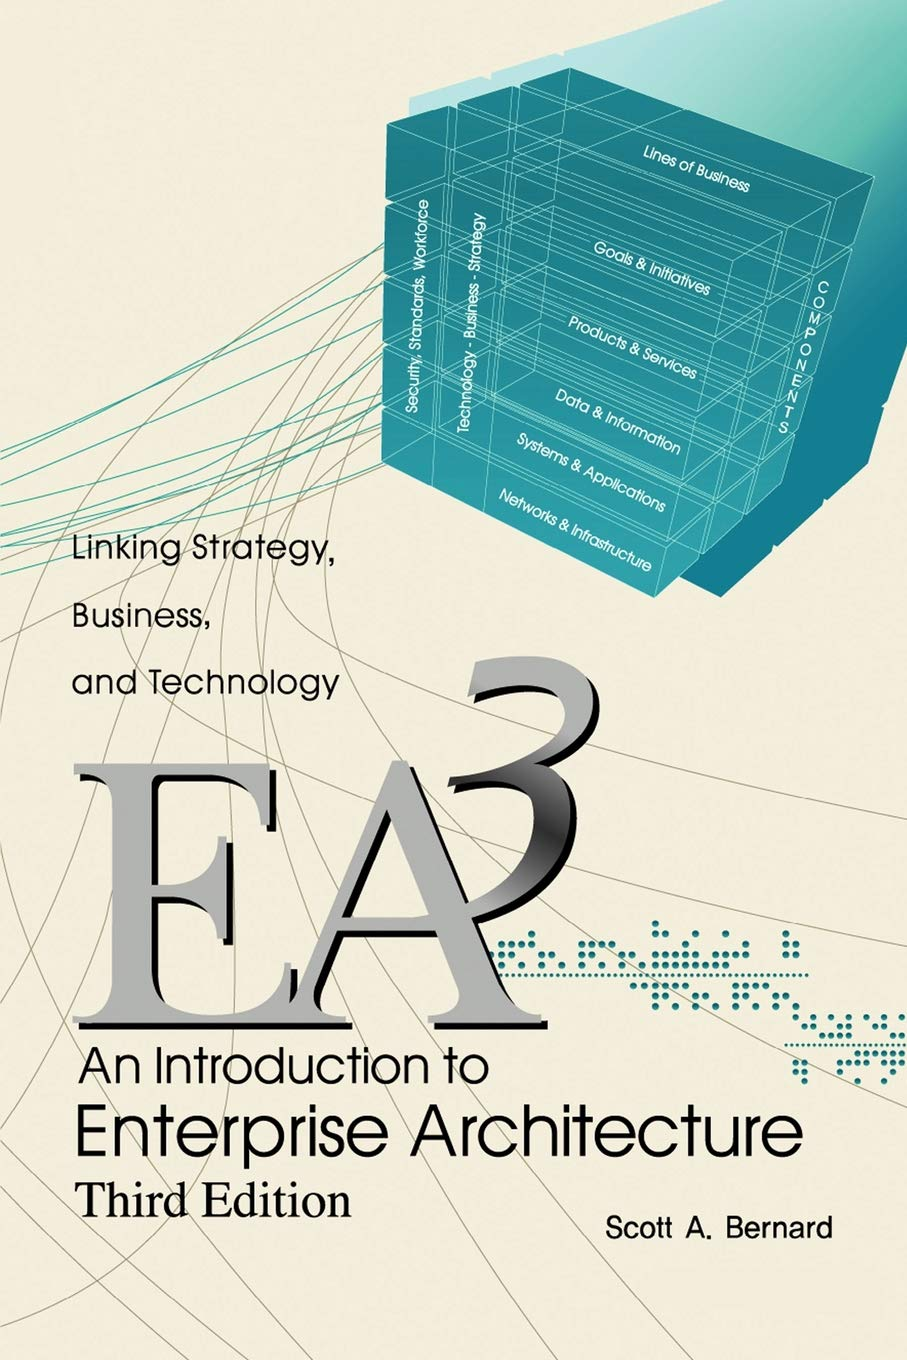
\includegraphics[width=1in]{img/cis476}} & \hangindent .4in \textbf{Textbook:} Bernard, S. A. (2012). An Introduction to Enterprise Architecture, 3rd Edition. AuthorHouse. ISBN-10: 1477258000. ISBN13: 978-1477258002. \\
%	\\
%	\adjustbox{valign=c}{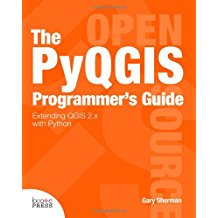
\includegraphics[width=1in]{img/cis430-2}} & \hangindent .4in \textbf{Textbook:} Sherman, G. (2014). The Pyqgis Programmer's Guide. Locate Press. ISBN-10: 0989421724 $\bullet$ ISBN-13: 978-0989421720. 
	%& \hangindent .4in Simulation Software: SAM 365 \& 2016 Assessments, Trainings, and Projects with MindTap Reader.
}